\documentclass{anstrans}
%%%%%%%%%%%%%%%%%%%%%%%%%%%%%%%%%%%
\title{Analysis of the LRA Reactor Benchmark Using Dynamic Mode Decomposition}
\author{Mohammad Abdo, Rabab Elzohery, and Jeremy A. Roberts}

\institute{
Department of Mechanical \& Nuclear Engineering, Kansas State University, Manhattan, KS 66506
}

% Optional disclaimer: remove this command to hide
%\disclaimer{Notice: this manuscript is a work 4of fiction. Any resemblance to
%actual articles, living or dead, is purely coincidental.}

%%%% packages and definitions (optional)
\usepackage{graphicx} % allows inclusion of graphics
\usepackage{booktabs} % nice rules (thick lines) for tables
\usepackage{microtype} % improves typography for PDF
\usepackage{lipsum}
\usepackage{tikz}
\newcommand{\SN}{S$_N$}
\renewcommand{\vec}[1]{\bm{#1}} %vector is bold italic
\newcommand{\vd}{\bm{\cdot}} % slightly bold vector dot
\newcommand{\grad}{\vec{\nabla}} % gradient
\newcommand{\ud}{\mathop{}\!\mathrm{d}} % upright derivative symbol
\DeclareMathOperator*{\argmin}{argmin}

\graphicspath{{../data/images/}}


\begin{document}
%%%%%%%%%%%%%%%%%%%%%%%%%%%%%%%%%%%%%%%%%%%%%%%%%%%%%%%%%%%%%%%%%%%%%%%%%%%%%%%%
\section{Introduction}

The next frontier of reactor modeling will require large-scale, full-core, transient models.
However, the herculean efforts involved will not likely be feasible for applications in which a system model must be executed for multiple system perturbations, e.g., design optimization and uncertainty quantification.
Hence, relatively  inexpensive surrogate models may be needed.

Given access to a high-fidelity model and corresponding solution, data-driven techniques can be used to generate surrogates without resorting to simplified physics or modifying the underlying implementation.  
One class of surrogates recently explored in the nuclear engineering community are those based on dynamic-mode decomposition.  
These past applications involved spatiotemporal dynamics that evolved relatively slowly in time, e.g., the evolution of isotopics \cite{} and decay-heat generation \cite{}.

Reactor transients exhibit much different dynamics.
With the restart of TREAT, preliminary efforts to apply generate surrogates based on gPC for uncertainty quantification have had some success \cite{}.
However, the surrogates generated lacked explicit time dependence and required substantial user development.

Presented here is the development of a data-driven surrogate based on dynamic-mode decomposition (DMD) to approximate time- and space-dependent fluxes and powers.
Specifically, a surrogate was produced for the 2-D LRA transient diffusion benchmark to illustrate the potential of the DMD approach. 
Whereas a conventional DMD surrogate cannot capture the rapid dynamics of the LRA transient, a composite surrogate constructed from a sequence of DMD surrogates defined for successive time windows proved more effective, the details of which are presented below.


\section{Dynamic Mode Decomposition}
\label{sec:backgound}

Interest in DMD has grown over the past decade for its ability to represent complex models with explicit temporal dynamics based on observed data alone.  
The basic algorithm was first proposed in the fluid-dynamics community by Schmid for the analysis of experimental data \cite{schmid:hal-01053394, schmid2010dynamic} but was swiftly developed by others in a variety of fields as has been thorougly detailed in the recent monograph by Kutz {\it et al.} \cite{kutzbook}.
Underlying the utility of DMD is its strong connection to Koopman theory and the Koopman operator, a linear, infinite-dimensional operator that acts on finite measurements of a nonlinear, dynamical system.
In other words, the Koopman operator provides the machinery to describe the evolution of observations of a nonlinear system in time, and DMD provides a finite-dimensional approximation to this operator.

\subsection{Conventional DMD} 

To motivate DMD, first consider the generic, dynamic problem defined by
\begin{equation}
  \frac{d{\vec{y} }(\vec{r},t)}{dt}=f(\vec{y},\vec{r},t) \, ,
\end{equation}
where ${\vec{y}} \in \mathbb{R}^{n}$ is the $n$-dimensional state vector at time $t$.  
Such a state vector may include neutron fluxes, local powers, temperatures, or functions of such quantities.
Suppose that the evolution of $\vec{y}$ can be well approximated by a relationship of the form  
\begin{equation}
 \frac{d{\vec{y}}(t)}{dt}=\mathcal{A}\vec{y} \, ,
\end{equation}
where the operator $\mathcal{A}$ may not be known explicitly. 
Suppose further that the quantities of interest are sampled at several times and organized as vector of a matrix, i.e.,
\begin{equation}
\mathbf{Y_0}=\left[\begin{array}{cccc}
| & | &   & | \\ 
{\vec{y_0}} &  {\vec{y_1}} & ... & {\vec{y_{m-1}}} \\ 
| & | &  & |
\end{array} \right]\, ,
\end{equation}
and
\begin{equation}
{\mathbf{Y_1}}=\left[\begin{array}{cccc}
| & | &  & | \\ 
{\vec{y_1}} &  {\vec{y_2}} & ... & {\vec{y_{m}}} \\ 
| & | &  & |
\end{array} \right] \, .
\end{equation}
where $m$ is the number of samples (often called snapshots).  
Then
\begin{equation}
  \vec{y_{k1}}=\mathbf{A}\vec{y_{k}}, \quad k = 0, 1, \ldots \, ,
\label{eq:snapshot_prop}
\end{equation}
where $\mathbf{A}=\exp(\mathcal{A}\Delta t)$.  
In general, no such operator $\mathbf{A}$ exists such that Eq.~(\ref{eq:snapshot_prop}) is satisfied, and instead, the relation is approximately satisfied by defining
\begin{equation}
\label{eq:AOpt}
    \mathbf{A}=\argmin\limits_{\mathbf{A}}\|\mathbf{Y_{1}} -\mathbf{AY_{1}}\|_F \, ,
\end{equation}
the solution of which is the pseudoinverse $\mathbf{A}=\mathbf{Y_1}\mathbf{{{Y}_{0}}^{\dagger}}$.
However, this matrix is large, and rather than compute it explicitly, the DMD exploits the low-rank approximation
\begin{equation}
\mathbf{\tilde{A}} = \mathbf{U_r^{H}AU_r} \, .
\end{equation}
Here, $\mathbf{U}_r$ aggregates the first $r$ columns of the left singular matrix resulting from the Singular Value Decomposition $ {\mathbf{A = U\Sigma V^T}}$, while $ \mathbf{U_r^{H}}$ is the Hermitian conjugate of $\mathbf{U}_r$.
The leading $r$ eigenvalues of $\mathcal{A}$ are inferred from the eigenvalues of $\mathbf{\tilde{A}}$. 
Once computed, the eigenvalues $\lambda_i$ of the discrete operator $\mathbf{A}$ can be transformed to the continuous frequencies $w_i$'s via $w_i=\log(\lambda_i)/\Delta t$.
The procedure is summarized in Algorithm \ref{algDMD}, in which $\vec{b}$ is the amplitude vector computed to satisfy the initial condition in the DMD basis (i.e., $\vec{b}={\boldsymbol{\Phi}^{DMD\dagger}} \vec{y_1}$).

TODO: add equations for the algorithm.

\subsection{Partitioned DMD}

%TODO: motivate need for time windowing and illustrate basic methodology.

%Maybe ``partitioned DMD''?  
DMD has major pitfalls, one is that the dynamic modes are non-orthogonal, and hence increasing the number of modes does not always enhance the the prediction as the added non-orthogonal mode might not be adding useful information but rather removing some information from the previous modes that might be vital for the system. 
That is why all the comparisons held between DMD and POD stated that the optimal number of dynamic modes in DMD is usually very few and as the number of modes is increased the prediction precision might reach an unacceptable threshold \cite{DMDvsPOD}. 
Although this is an undesirable quality that requires careful analysis to pick the proper rank, it is a motivation for the proposed idea. 
Second, is the statement declared by many scientists about possible deficiency of DMD to capture transient effects. 
And the reason for that is that for fast transient, the space spanned by the snapshots is rapidly changing and deviating in a rather short time increments. 
This motivated the idea of partitioned DMD. 
If our dynamics can be broken into portions where the time scales within each portion are comparable, but are very different from other portions. 
And/or if the first time trajectory had an intrinsic DMD rank that is different than the second portion/trajectory, that is the case where all the basis coming from the snapshots (and hence a full rank surrogate) in an interval are needed in the interval with the most aggressive and rapid dynamical change, whereas we do not need that before and after that time period. 
Those cases motivated the inspection of the partitioned DMD surrogate where the whole analysis time is broken into partitions, each of which is dealt with separately, to construct a DMD surrogate. 
This allows to pick different ranks for each interval and also to pick the appropriate dynamic mode scaling, since this performs differently with how slow/fast are your dynamics, which means that the interval with slow dynamics might use Eq.~\ref{eq:bOpt}, whereas for other intervals, the original initial condition projected on the DMD modes (i.e., $\vec{b}={\boldsymbol{\Phi}^{DMD\dagger}} \vec{y_0}$) might be sufficient.


\section{LRA Benchmark}
\label{sec:application}

% Describe the numerical specific of LRA, the perturbations used, and why they are of interest.

The two-dimensional, two-group diffusion LRA benchmark problem is a simplified, quarter-core, BWR model subject to a control-rod ejection with adiabatic heating.
Although complete details can be found elsewhere \cite{}, the basic assembly layout is shown in Fig.~\ref{fig:lra_core}.
To produce the time-dependent snapshots of Eq.~({eq:xxx}), the determinstic transport code {\tt Detran} \cite{} was used to solve the time-dependent diffusion equations.  
A mesh-centered, finite-volume discretization was used with a 7.5 cm mesh throughout.
A second-order, backward-difference temporal discretization was used with a fixed 0.01 s step size.  
The solution at each time step was converged using fixed-point iteration.
The discretization used is far from numerically converged, but it produces a sufficiently rich set of data for demonstration.

\begin{figure}
\begin{tikzpicture}[scale=.4]

\begin{scope}<->;

% GRID
  \draw[step=1.5cm,gray,very thin, dashed,opacity=0.4] (0, 0) grid (16.5,16.5);

% AXES
  \draw[black, thick, ->] (0, 0) -- (17,  0) node[right] {$x$};
  \draw[black, thick, ->] (0, 0) -- ( 0, 17) node[above] {$y$};

% Material 1 regions 

  \node[font=\large] at (5.25, 5.25) {1};
  
% Material 2 regions
  \draw[black, thick] (0, 1.5) -- (1.5, 1.5);
  \draw[black, thick] (1.5, 0) -- (1.5, 1.5);
  \node[font=\large] at (0.75, 0.75) {2};
  
  \draw[black, thick] ( 7.5, 0.0) -- ( 7.5, 1.5);
  \draw[black, thick] (10.5, 0.0) -- (10.5, 1.5);
  \draw[black, thick] ( 7.5, 1.5) -- (10.5, 1.5);
  \node[font=\large] at (9.0, 0.75) {2};

  \draw[black, thick] ( 0.0,  7.5) -- ( 1.5,  7.5);
  \draw[black, thick] ( 0.0, 10.5) -- ( 1.5, 10.5);
  \draw[black, thick] ( 1.5,  7.5) -- ( 1.5, 10.5);
  \node[font=\large] at ( 0.75, 9.0) {2};
  
  \draw[black, thick] ( 7.5,  7.5) -- ( 7.5, 10.5);
  \draw[black, thick] ( 7.5,  7.5) -- (10.5,  7.5);
  \draw[black, thick] (10.5, 10.5) -- ( 7.5, 10.5);
  \draw[black, thick] (10.5, 10.5) -- (10.5,  7.5);
  \node[font=\large] at ( 9.0, 9.0) {2};

% Material 3 regions
  \draw[black, thick] (10.5,  0.0) -- (10.5, 10.5) -- (13.5, 10.5) --  (13.5,  0.0) -- (10.5,  0.0);
  \node[font=\large] at ( 12.0, 3.75) {3}; 
  \draw[black, thick] (0.0, 10.5) -- (10.5, 10.5) -- (10.5, 13.5) -- (0.0, 13.5) --  (0.0, 10.5);
  \node[font=\large] at ( 3.75, 12.0) {3}; 
  
% Material 4 regions  
  \draw[black, thick] ( 12,  12) -- ( 12, 10.5) -- (10.5, 10.5) -- (10.5,  12) -- ( 12,  12);
  \node[font=\large] at ( 11.25,11.25) {4};

   
% Material 5 regions
  \draw[black, thick] ( 16.5,  0.0) -- (16.5, 16.5);
  \draw[black, thick] (  0.0, 16.5) -- (16.5, 16.5);
  \node[font=\large] at (15.0, 15.0) {5};
 
% Perturbed regions
  \def\eps{0.125}
%   \draw[black, thick, dashed] (10.5\eps, 7.5\eps) -- (10.5\eps, 10.5-\eps) -- (13.5-\eps, 10.5-\eps) -- (13.5-\eps, 7.5\eps) --  (10.5\eps, 7.5\eps);

  %\draw[black, thick] ( 12,  12) -- (10.5,  12);
  %\draw[black, thick] (10.5, 10.5) -- ( 12, 10.5);
  %\draw[black, thick] (10.5, 10.5) -- (10.5,  12);
  \node[font=\large] at (12,9) {R};
 
% ticks
  \foreach \x/\xtext in {15, 75, 105, 120, 135, 165}
      \draw[black,xshift=0.1*\x cm] (0,.3) -- (0,0) node[below] {$\xtext$};
  \foreach \y/\ytext in {15, 75, 105, 120, 135, 165}
      \draw[black,yshift=0.1*\y cm] (.3,0) -- (0,0) node[left] {$\ytext$};
\end{scope}
\end{tikzpicture}
\caption{Schematic of LRA benchmark.  Region numbers indicate material assignment.  Region R is the the ejected rod.  A 15 cm coarse mesh for individual assemblies is overlaid.}
\label{fig:lra_core}
\end{figure}

The initial condition for the transient was computed by solving the steady-state equations, for which the $k_{\text{eff}}$ was found to be 0.9975.
The transient was executed up to 3 seconds.
The space and time discretization employed results in a local (fine-mesh) power distribution of $X \times X$ values recorded at Y times.


\section{Surrogate Generation and Performance}

The partioned DMD algorithm

All DMD surrogates were constructed in Python using modification of {\tt PyDMD} \cite{}.


\begin{figure*}[t!]
 \centering
 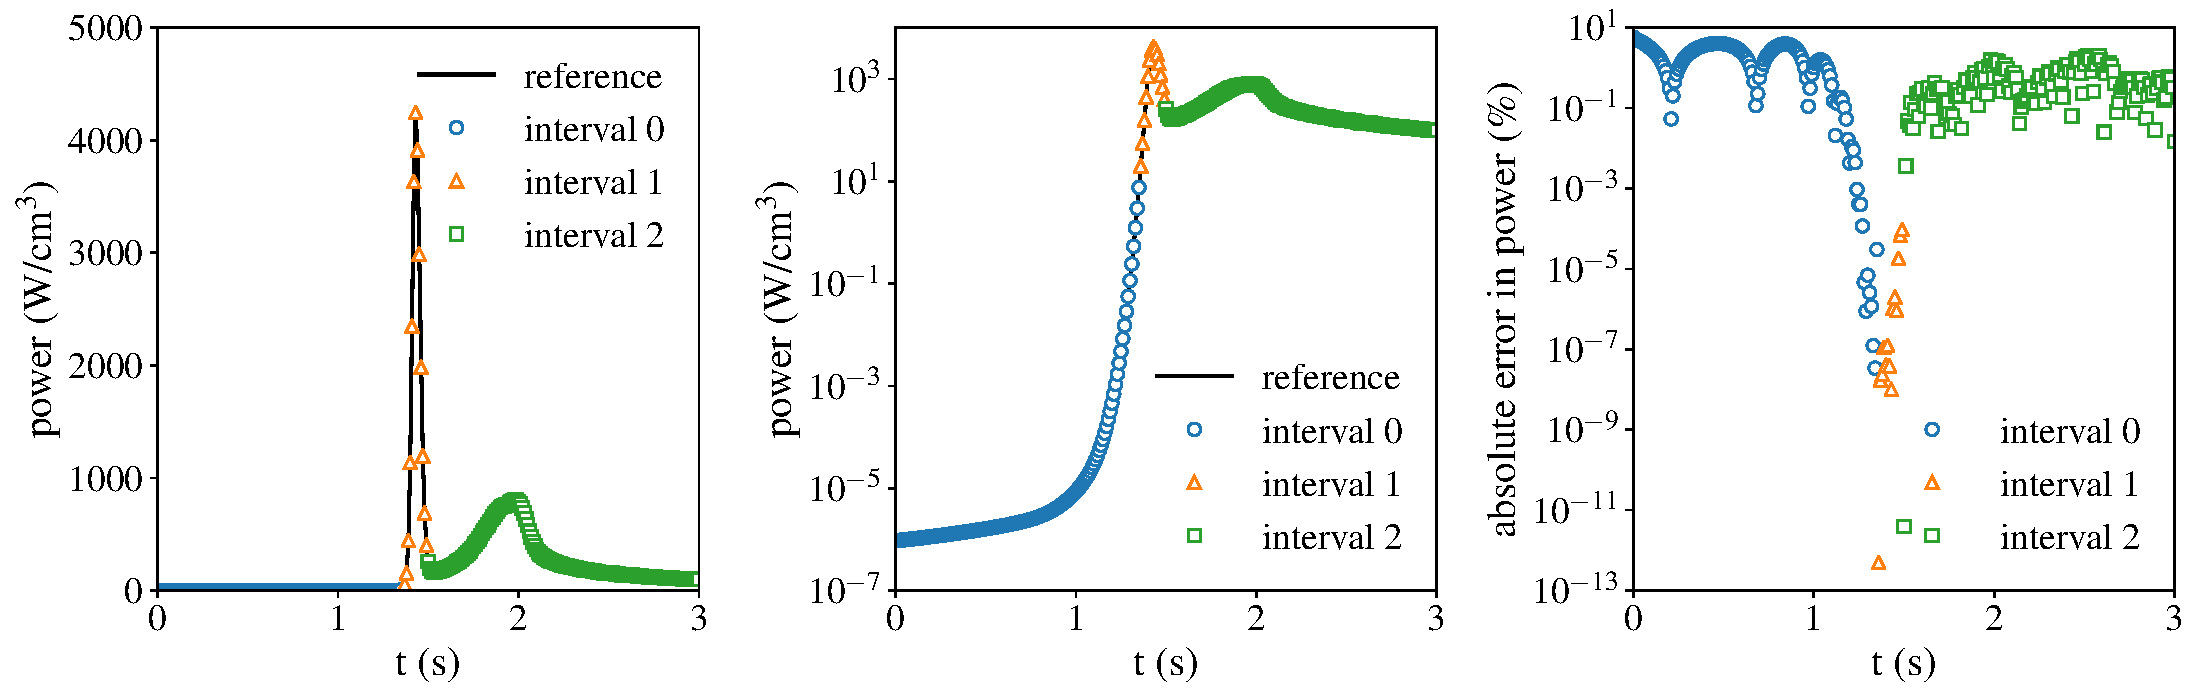
\includegraphics[width=\textwidth]{corepower}\\
   \caption{Left and center: reference and approximate core power density; right: corresponding absolute, relative error.}
  \label{fig:corepower}
\end{figure*}


\section{Conclusions}

A DMD-based surrogate was shown to represent the spatiotemporal dynamics of the LRA benchmark accurately when by produced by a sequence of individual DMD surrogates in time. 
The surrogate was shown to be sensitive to the time partioning.
Work is ongoing to mitigate this sensitivity and to provide an automated way to select the number of partitions and their boundaries.

\section{Acknowledgments}

The material presented is based on work supported in part by the U.S. Nuclear Regulatory Commission, Office of Nuclear Regulatory Research, under award number NRC-HQ-60-15-G-0004.

%%%%%%%%%%%%%%%%%%%%%%%%%%%%%%%%%%%%%%%%%%%%%%%%%%%%%%%%%%%%%%%%%%%%%%%%%%%%%%%%
\bibliographystyle{ans}
\bibliography{bibliography}
\end{document}
